\chapter{Introduction} \label{chap_introduction}

Sinds the early days there have been challenges with creating and maintaining stable and
evolvable software. On the one hand, this is caused by constantly evolving requirements as
new business opportunities, technologies, methodologies, and best practices are developed
to meet the demands of modern corporate environments. On the other hand, changing software
can lead to deterioration in stability and evolvability, which can negatively impact the
quality of these systems. \textcite{lehman_programs_1980} has described this as one of his
laws of software evolution: The balance between the forces driving new requirements and
those that slow down progress. These challenges have been recognized by the following
pioneers in software engineering. 

\textcite{d_mcilroy_nato_1968} proposed a vision where the systematic reuse of software
building blocks should lead to more reuse. \textcite{d_mcilroy_nato_1968} quoted
\enquote{The real hero of programming is the one who writes negative code}, i.e. when a
change in a program source makes the number of lines of code decrease ('negative' code),
while its overall quality, readability or speed improves
\footnote{\url{https://en.wikipedia.org/wiki/Douglas_McIlroy}}. Perhaps very early concepts
of modular software constructs?

\textcite{dijkstra_letters_1968} argued against using unstructured control flow in
programming and advocated for using structured programming constructs to improve the
clarity and maintainability of the source code. He advocated structured programming
techniques that improved the modularity and evolvability of software artifacts.

\textcite{parnas_criteria_1972} continued with the principle of information hiding. He
stated that design decisions used multiple times by a software artifact should be
modularized to reduce complexity. 

Various programming paradigms, including procedural, object-oriented, and functional
programming, have emerged to enhance software programming capabilities that contribute to
stability and evolvability \parencite{mannaert_normalized_2016}. These paradigms have
impacted modern programming languages, such as Java and C\#, enabling the development of
more modular and evolvable software architectures.

Design principles, patterns, and theorems are, on top of all, additional measures to
enhance the modularity, stability, and evolvability of software artifacts. As a junior
software engineer, I was always intrigued by the concepts of quality and maintainable code
and quickly got introduced to the \gls{solid} principles. And later on with the complete
design approach derived from \gls{ca}. Starting my Master's degree, I got an
inspiring introduction from Jan Verelst and realized quality and maintainability were
essentially all about the concepts of stability and evolvability. For me, it was very
interesting that the \gls{ns} Theory is supported by empirical scientific evidence.
Although I'm not that active anymore in the field of software engineering, I immediately
knew the topic of my research. it is still a big passion of mine.

Given my experience with \gls{ca}, and what I was learning from \gls{ns} Theory, I noticed
a lot of similarities, but also some big differences. In early investigations, I found
overlapping characteristics. But it seemed there were also a couple of differences. I
wanted to know if the design approaches could be used in conjunction with each other,
perhaps bettering the result of stable and evolvable software.

Java SE has primarily been used for case studies in order to develop the Normalized
Systems Theory \parencite{oorts_building_2014, de_bruyn_enabling_2018}. Although
sufficient in Java, I was pleased to read that both software design approaches have
formulated their modular structures independent of any programming technology
\parencite{mannaert_normalized_2009,robert_c_martin_clean_2018}. So I was free to use my
favorite programming language C\# to create a software artifact that supported my
research, igniting my passion for programming again. 

Based on my early investigations of both design approaches I hypothesized that they can be
used in conjunction with each other. Consequently, an artifact that is designed based on
the principles of Clean Architecture will lead to a highly modular, stable, and evolvable
C\# artifact that does not contradict a design based on the Normalized Systems theorems.

\begin{figure}[H]
    \centering
    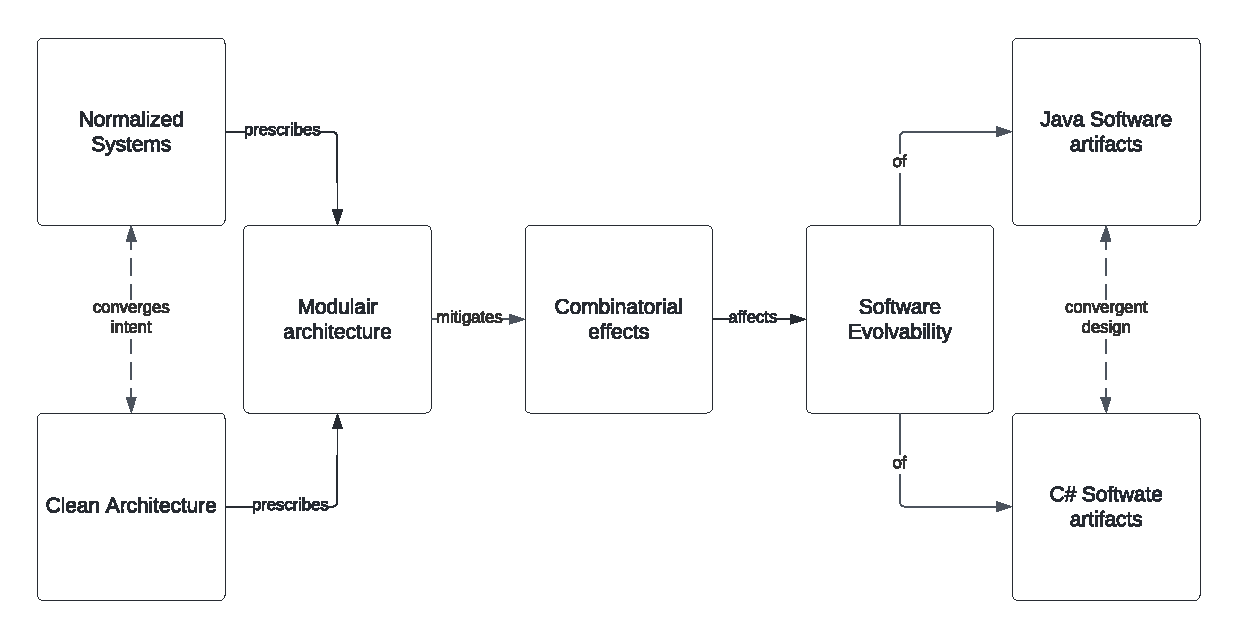
\includegraphics[width=0.8\textwidth]{figures/hypothesis.pdf}
    \caption[The hypothesis]{The hypothesis}
    \label{fig_hypothesis}
\end{figure}

\section{Introduction to Normalized Systems} \label{sec_inro_ns}

The \gls{ns} Theory is a scientific approach to creating software systems based on the
laws for software evolvability. \gls{ns} has contributed to a documented track record of
achieving software stability in a scientific environment. Effectively, it prevents the
accumulation of required changes required on the implementation of new requirements
\parencite[]{mannaert_normalized_2009}. 

\citeauthor[]{mannaert_normalized_2009} have formulated the Theories of \gls{ns} as rigid
structures (elements) that lead to a modular architecture with low coupling and high
cohesion. The resulting software architecture will be designed to cope with future
changes.
\section{Introduction to Clean Architecture} \label{sec_into_ca}

\gls{ca} is the accumulation of more than half a century of coding, designing, and
architecting software systems by \citeauthor*[]{robert_c_martin_clean_2018}. He published
his experience in his book \citetitle*[]{robert_c_martin_clean_2018} in
\citeyear[]{robert_c_martin_clean_2018}. In this book, he states that creating a software
artifact is not that difficult. However, creating stable and maintainable software
artifacts is a skill that requires a lot of knowledge, skill, dedication, and time.

The book aims for a software architecture that minimizes the human resources required to
build and maintain the information system. Like \gls{ns}, it has a prescribed design of
software elements that will lead to a modular architecture with low coupling and high
cohesion. Additionally, the book refers to a set of design principles that prescribes the
way those elements should be structured, or interact with each other
\parencite{robert_c_martin_clean_2018}.

\section{Research Objectives} \label{sec_research_objectives}

In this Design Science Research, we will shift the focus from Research Questions to
Research Objects. The primary goal of this research is to determine the degree of
convergence of \gls{ca} with the \gls{ns} Theory. In order to achieve this goal, the
research is divided into the following objectives:

\begin{enumerate}
    \item \textbf{Literature Analysis} \newline
    Conduct a literature review of \gls{ca} and \gls{ns}, focusing on their
    fundamental elements, principles, and real-world case studies. This review will
    provide a solid foundation for understanding the underlying concepts and their
    practical implications.
    
    \item \textbf{Architectural Desing} \newline
    Create an Architectural Design fully and solely based on \gls{ca}. Implement the
    findings of the Literature Review in the Design. This design will be the basis for
    the Artifact Development.

    \item \textbf{Artifact Development} \newline
    Construct two artifacts that facilitates the study on the convergence
    between \gls{ca} and \gls{ns} Theories.
    \begin{enumerate}[label*={\arabic*.}]
        
        \item \textbf{Expander framework \& Clean Architecture Expander} \newline        
        These two components will be designed and implemented  based on the \gls{ca}
        design. The Clean Architecture Expander will enable the parameterized
        instantiation of software systems that adhere to the principles and design of
        \gls{ca}. The Expander framework serves as a supporting system for the expander,
        loading and orchestrating dependencies and models and executing the expander.
        
        \item \textbf{Expanded Clean Architecture artifact} \newline
        The expanded artifact will facilitate the analysis of a RESTful API implementation
        and its alignment with the \gls{ca} principles and design.
        
    \end{enumerate}
    
    \item \textbf{Analysis of combinatorics} \newline
    Analyze the artifacts to determine if any combinatorial effects occur due to following
    the principles and architectural approach of \gls{ca}.
\end{enumerate}
%\input{chapters/introduction/sections/researchquestion}
\section{Research method} \label{sec_research_method}

This research is a Design Science Method and relies on the Engineering Cycles as described
by \textcite{wieringa_design_2014}. The engineering cycle provides a structured approach
to developing the required artifacts to analyze the design problem.

\begin{figure}[H]
    \centering
    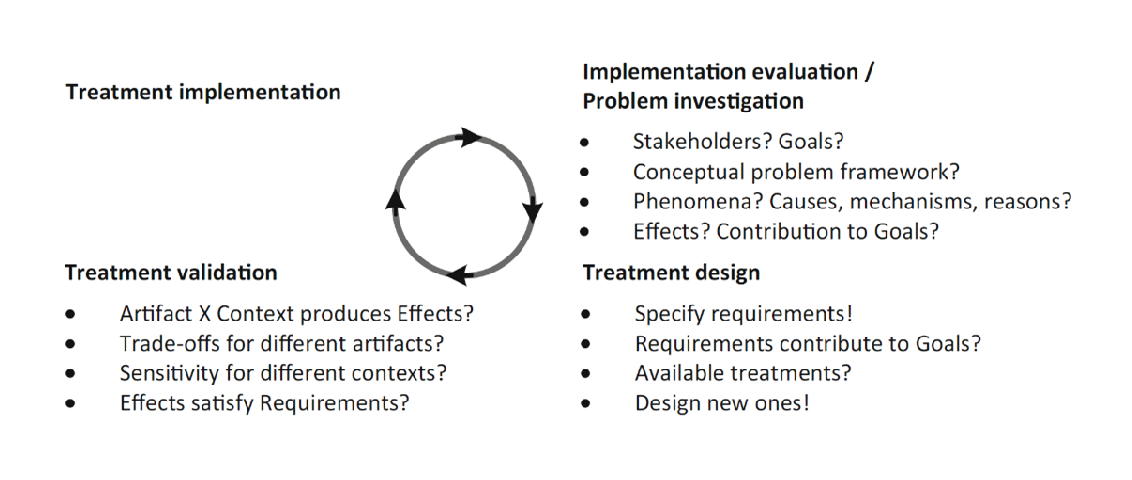
\includegraphics[width=1\textwidth]{figures/engineering_cycle.pdf}
    \caption[Engineering cycle]{The Engineering Cycle of \textcite{wieringa_design_2014}}
    \label{fig_engineering_cycle}
\end{figure}

In the course of this research, a significant component has been the development of a
tangible software artifact, providing a real-world illustration of the convergence between
Clean Architecture and Normalized Systems. \textcite{hevner_design_2004} proposed a
framework for research in information systems by introducing the interacting relevance and
rigor cycles.

Figure \ref{fig_dsr} depicts a specialization of the Design Science Framework of
\textcite{hevner_design_2004}. The rigor cycle comprises the theories and knowledge from
\gls{ns} and \gls{ca}, supplemented by the rigorous knowledge of modularity, evolvability,
and stability of software systems. The relevance cycle represents the business needs of
the stakeholders. The research requirements are described as research objectives.

\begin{figure}[H]
    \centering
    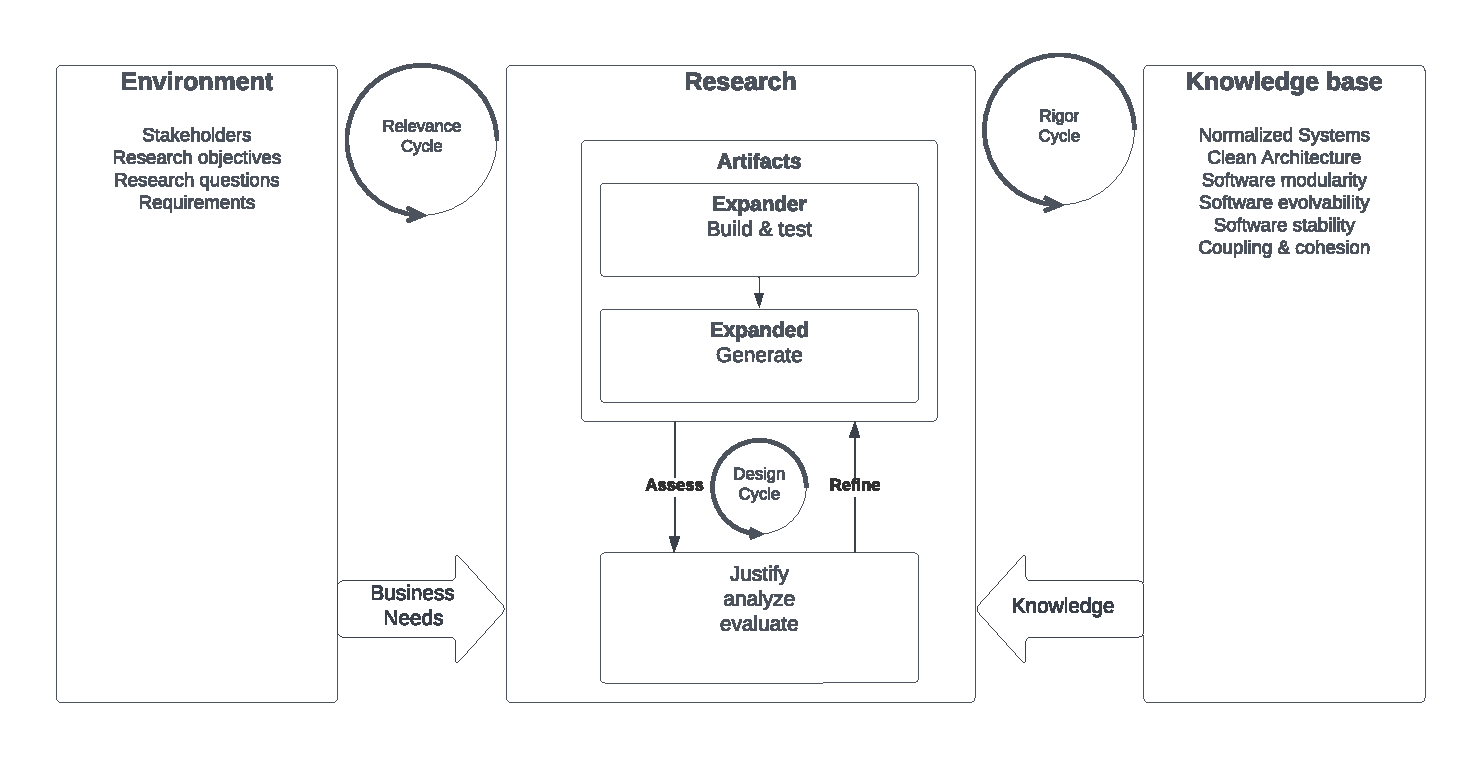
\includegraphics[width=1\textwidth]{figures/rigor_relevance_cycle.pdf}
    \caption[Design Science Framework for IS Research]{The Design Science Framework for IS Research}
    \label{fig_dsr}
\end{figure}
\section{Thesis outline} \label{sec_structure}

The structure of this thesis reflects the research methodology described in the previous
section \ref{sec_research_method}. Chapter \ref{chap_theoreticalbackground} presents the
theoretical backgrounds of both \gls{ns} and \gls{ca}, discussing important
characteristics and requirements of software stability, as well as the principles and
architectures proposed by both development approaches. Chapter \ref{chap_requirements}
focuses on the requirements relevant to this research. It is divided into two sections:
section \ref{sec_research_requirements} outlines the research requirements, describing the
requirements necessary for conducting the research, while section
\ref{sec_artifact_requirements} details the artifact requirements, laying out the
requirements relevant to the artifacts contributing to this research. Chapter
\ref{chap_designing_artifacts} describes all the characteristics of the design artifacts.
Chapter \ref{chap_evaluation} evaluates the research results, discussing the impact of
using CA on NS. The conclusion of this research is presented in the final chapter, Chapter
\ref{chap_conclusions}.